%% 
%% Copyright 2007, 2008, 2009 Elsevier Ltd
%% 
%% This file is part of the 'Elsarticle Bundle'.
%% ---------------------------------------------
%% 
%% It may be distributed under the conditions of the LaTeX Project Public
%% License, either version 1.2 of this license or (at your option) any
%% later version.  The latest version of this license is in
%%    http://www.latex-project.org/lppl.txt
%% and version 1.2 or later is part of all distributions of LaTeX
%% version 1999/12/01 or later.
%% 
%% The list of all files belonging to the 'Elsarticle Bundle' is
%% given in the file `manifest.txt'.
%% 
%% Template article for Elsevier's document class `elsarticle'
%% with harvard style bibliographic references
%% SP 2008/03/01

%% \documentclass[preprint,12pt,authoryear]{elsarticle}

%% Use the option review to obtain double line spacing
%% \documentclass[authoryear,preprint,review,12pt]{elsarticle}

%% Use the options 1p,twocolumn; 3p; 3p,twocolumn; 5p; or 5p,twocolumn
%% for a journal layout:
%% \documentclass[final,1p,times,authoryear]{elsarticle}
%% \documentclass[final,1p,times,twocolumn,authoryear]{elsarticle}
%% \documentclass[final,3p,times,authoryear]{elsarticle}
%% \documentclass[final,3p,times,twocolumn,authoryear]{elsarticle}
%% \documentclass[final,5p,times,authoryear]{elsarticle}
\documentclass[final,5p,times,twocolumn,authoryear]{elsarticle}

%% For including figures, graphicx.sty has been loaded in
%% elsarticle.cls. If you prefer to use the old commands
%% please give \usepackage{epsfig}

%% The amssymb package provides various useful mathematical symbols
\usepackage{amssymb}
%% The amsthm package provides extended theorem environments
%% \usepackage{amsthm}

%% The lineno packages adds line numbers. Start line numbering with
%% \begin{linenumbers}, end it with \end{linenumbers}. Or switch it on
%% for the whole article with \linenumbers.
%% \usepackage{lineno}



\usepackage[utf8]{inputenc}
\DeclareFixedFont{\ttb}{T1}{txtt}{bx}{n}{9} % for bold
\DeclareFixedFont{\ttm}{T1}{txtt}{m}{n}{9}  % for normal
% Defining colors
\usepackage{color}
\definecolor{deepblue}{rgb}{0,0,0.5}
\definecolor{deepred}{rgb}{0.6,0,0}
\definecolor{deepgreen}{rgb}{0,0.5,0}


\usepackage{listings}

% Python style for highlighting
\newcommand\pythonstyle{\lstset{
language=Python,
backgroundcolor=\color{white}
basicstyle=\ttm,
otherkeywords={self},            
keywordstyle=\ttb\color{deepblue},
emph={MyClass,__init__},          
emphstyle=\ttb\color{deepred},    
stringstyle=\color{deepgreen},
commentstyle=\color{red}
frame=tb,                         
showstringspaces=false            
}}

% Python environment
\lstnewenvironment{python}[1][]
{
\pythonstyle
\lstset{#1}
}
{}

\journal{Astronomy and Computing}

\begin{document}

\begin{frontmatter}

%% Title, authors and addresses

%% use the tnoteref command within \title for footnotes;
%% use the tnotetext command for theassociated footnote;
%% use the fnref command within \author or \address for footnotes;
%% use the fntext command for theassociated footnote;
%% use the corref command within \author for corresponding author footnotes;
%% use the cortext command for theassociated footnote;
%% use the ead command for the email address,
%% and the form \ead[url] for the home page:
%% \title{Title\tnoteref{label1}}
%% \tnotetext[label1]{}
%% \author{Name\corref{cor1}\fnref{label2}}
%% \ead{email address}
%% \ead[url]{home page}
%% \fntext[label2]{}
%% \cortext[cor1]{}
%% \address{Address\fnref{label3}}
%% \fntext[label3]{}

\title{LightCurvesClassifier: Searching in light curves}

%% use optional labels to link authors explicitly to addresses:
%% \author[label1,label2]{}
%% \address[label1]{}
%% \address[label2]{}

\author{ Martin Vo }

\address{ Czech Republic }

\begin{abstract}
%% Text of abstract

\end{abstract}

\begin{keyword}
Light Curves \sep Data Mining \sep Machine Learning \sep SAX
%% keywords here, in the form: keyword \sep keyword

%% PACS codes here, in the form: \PACS code \sep code

%% MSC codes here, in the form: \MSC code \sep code
%% or \MSC[2008] code \sep code (2000 is the default)

\end{keyword}

\end{frontmatter}

%% \linenumbers

%% main text
\section{Introduction}
\label{}

We are living in the world of Big Data - huge astronomical surveys which represent immeasurable possibilities of analyzing of their data. Despite of huge spectroscopic surveys, light curves are still dominant source of information about the universe. There are many
teams which work on searching for certain objects, but there is no complex tool which has a potential to make this task much more easier and efficient by using modern machine learning methods. Furthermore  \textit{Light Curve Classifier} is capable to be easily extended by users and become universal tool for classifying stars not only by light curves.


%% The Appendices part is started with the command \appendix;
%% appendix sections are then done as normal sections
%% \appendix

\section{Program}

The \textit{Light Curve Classifier} is Python package which for classifying, analyzing and downloading light curves. There are several database connectors to OgleII \citet{ogleII}, Kepler Archive \cite{kepler}, Macho \cite{macho} and CoRoT \cite{corot} databases. Filtering of stars can be executed directly on these databases or locally from light curve files. 

The main purpose of the program is to search thru big storage of light curves and looking for certain patterns of light curves or attributes of star objects. It is done by various filters and supervised machine learning methods.

\subsection{How to filter stars?}

There are many attributes of stars which can be evaluated - color indexes, statistical values of their light curves, dissimilarity of inspected star to a template, temperatures etc. These tasks are reflected in an implementation of particular filters. Many of them are already included in the package, but there is no limitation to easily implement new ones (see \ref{new_imple}).

\subsection{How to teach filters?}

Each filter assigns an unique value to particular stars. For example color index, variance of a light curve etc. These values can be considered as coordinates in $N$ dimensional space ($N$ is number of "inner variables"). Filters are connected to helpers - "deciders", they tell to filters if star with certain coordinates can pass thru the filter. Basically, "deciders" are supervised methods which are able to learn on train sample and then estimate probability of membership of inspected star to searched group. During learning "decider" receiving coordinates of labeled stars from filters - sample of searched stars and a contamination sample. These coordinates serve as schoolbook for "deciders" (as is it shown on \ref{histvario}).

\begin{figure}
\label{histvario}
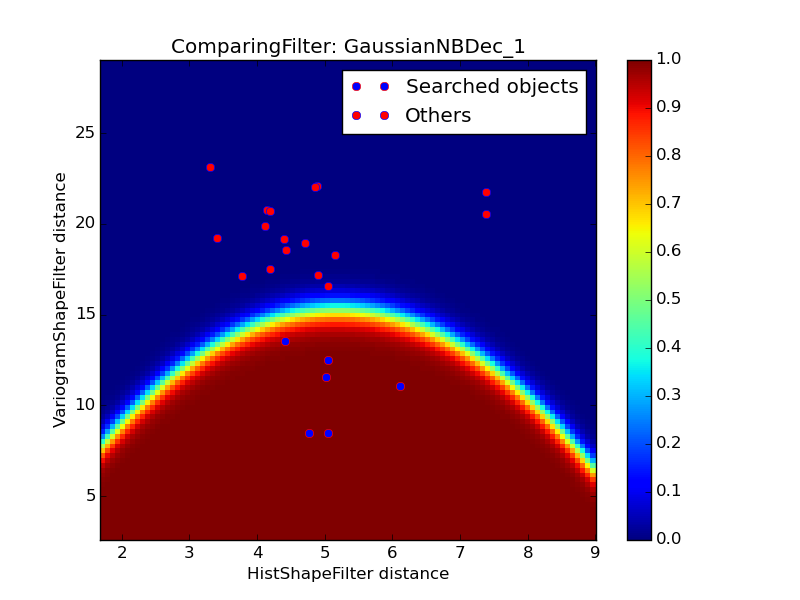
\includegraphics[scale=0.5]{figures/histvario.png}[H]
\caption{Histogram-variogram space. Position of star objects represent dissimilarity from template sample. On the background is plotted probability distribution created by "decider" - in this example Gaussian Naive Bayes method.}
\end{figure}


Global parameter for filtering is treshold which represents percentage value as the minimal confidence level which is needed to pass thru particular filters.


\subsection{What is the most optional filter parameters?}
Also filters can have some parameters which have to be tuned, but it is not necessary to do any research to find them, but all is done automatically during "learning" phase - all combinations of parameters are estimated and the best ones are used for constructing the filter. Each parameters combination returns statistical values (true/false positive/negative rates) which can be used for implementing own function (in settings file) which decides what is the most optional combination. Default function is precision $PPV$ defined as:

\begin{equation}
PPV = \frac{TP}{TP + FP }.
\end{equation}
%
where $TP$ is true positive and $FP$ is false positive.

\section{Usage}

Progress schema:

\begin{enumerate}
\item Prepare combinations of parameter for tuning a filter
\item Prepare queries for a database
\item Make filter
\item Execute systematic search in a database
\end{enumerate}
%
Each step corresponds with one execution of a script.

\subsection{ Example }

In this example we would like to search in  Ogle archive of light curves \cite{ogleII} and look for light curves with shape similar to our sample of light curves. For this purpose we can use \textit{Comparing Filter} which is designated to compares two light curves and calculate their dissimilarity. In this particular task we will compare shapes of light curves itself. However it is possible to compare derived data series as histograms, variograms etc.  \textit{Comparing Filter} transforms time series into symbolic representation via SAX method \cite{sax} and compares two words. 

Before running systematic filtering in our database, we have to find the most optional parameters of the filter. In case of \textit{Curve Shape Filter} there are two parameters - length of alphabet and dimension reduction ratio (number of bins per day). Let's generate file of parameters combinations:

\begin{lstlisting}
./prepare_query.py
	-o params_comb.txt
	-p lc_days_per_bin -r 50:150:15	
	-p lc_alphabet_size -r 8:19:2 
	
\end{lstlisting}
%
Also we can generate query file for searching our database:

\begin{lstlisting}
./prepare_query.py
	-o ogle_query.txt
	-p target -r lmc
	-p starid -r 1:100000
	-p field_num -r 1:20
\end{lstlisting}
%
Now we can train our filter and find the most optional parameters by one command:

\begin{lstlisting}
./make_filter.py
	-i params_comb.txt	
	-s my_lcs_folder
	-c contamination_lcs_folder
	-o my_filter
	-l my_logs_folder
	-f ComparingFilter
	-d NeuronDecider	
\end{lstlisting}

From all combinations of parameters in \textit{params\_comb.txt} the most optional is stored as filter object file \textit{my\_filter}. Learning is managed by \textit{NeuronDecider} and train sample contains light curves stored in \textit{my\_lcs\_folder} and \textit{contamination\_lcs\_folder}. Output logs and images are saved into \textit{my\_logs\_folder}. 

Finally we can use created filter and run systematic filtering in the database:

\begin{lstlisting}
./filter_stars.py
	-i query_ogle.txt
	-o found_lcs
	-d KeplerArchive
	-f my_filter	
\end{lstlisting}

Light curves of stars passed thru filtering and log file about filtering are saved into \textit{found\_lcs} directory.

 

\section{Implemented modules} 


There are three groups of modules intended to be be used and extended:

\begin{enumerate}
\item Database connectors
\item Filters
\item Deciders
\end{enumerate}

Lots of them are already implemented, but it is possible and encouraged to implement new ones. All theses three categories has own API which lays demands on new classes. It guarantees compatibility of all new modules with rest of the program. See \ref{new_imple} chapter for more (but still brief) details.


\subsection{ Database connectors }
\label{ filtering_sec }

Database connectors can be used both from command line and by coding:

\begin{lstlisting}[caption = {Query MACHO database by scripts}, label={colors}]
./prepare_query.py
	-o query.txt
	-p ra -r "0.4797"
	-p dec -r "-67.1290"
	-p delta -r "10"
	
./filter_stars.py
	-i query.txt
	-o save_folder
	-d "MachoDb"
\end{lstlisting}

Second example:

\begin{lstlisting}[caption = {Query MACHO database by scripts}, label={colors}]
./prepare_query.py
	-o query.txt
	-p Field -r "1"
	-p Tile -r "3441"
	-p Seqn -r "25"
	
./filter_stars.py
	-i query.txt
	-o save_folder
	-d "MachoDb"
\end{lstlisting}

Same result can be achieved by few lines in Python:

\begin{python}
querie = [{"ra": 0.4797, "dec": -67.1290, "delta": 10},
         {"Field": 1 , "Tile": 3441, "Seqn": 25}]
client = StarsProvider().getProvider( obtain_method = "MachoDb", obtain_params = queries)
stars = client.getStarsWithCurves()
[star.saveStar("save_folder") for star in stars]
\end{python}

\subsubsection*{OgleII BVI database}

Optical Gravitational Lensing Experiment provides light curves in I-band of more then 40 millions of objects in LMC, SMC and galactic bulge.

\subsection*{CoRoT Archive}

Space mission dedicated to exoplanet search and stellar physics. Light curve files are saved into \cite{CoRoT}, but the catalog is stored in Vizier \cite{vizier}. Actually there are two separated tables: \textit{Bright stars} (171 rows) and \textit{Faint stars} (177382 rows). Light curves have no calculated magnitudes, but just fluxes. 

\subsubsection*{Kepler Archive}

Connector to Kepler Objects of Interest catalog \cite{kepler} and its light curves from MAST \cite{mast}. 

\subsubsection*{MACHO}

The main aim of MACHO surveys is searching for microlensing events, but there are huge by-product

\subsubsection*{File Manager}

This connector manages light curve files stored locally.

\subsubsection*{Local Db Client}

This connector manages connections to local databases. 

***

\subsection{ Learning }
\label{ learning_sec }



\subsection{ Getting light curves }
\label{connectors_sec }

The crucial step for searching in light curves is to obtain any. There are several astronomical databases with web interface which allow to download light curves, but it is a nightmare to use them programmatically for a systematic searching. The package provides few implementations 



\section{New modules}
\label{new_imple}

%% \section{}
%% \label{}













%% If you have bibdatabase file and want bibtex to generate the
%% bibitems, please use
%%
\bibliographystyle{elsarticle-harv} 
\bibliography{LightCurvesClassifier}

%% else use the following coding to input the bibitems directly in the
%% TeX file.

%%% \begin{thebibliography}{00}

%% \bibitem[Author(year)]{label}
%% Text of bibliographic item

%%% \bibitem[ ()]{}

%%% \end{thebibliography}
\end{document}

\endinput
%%
%% End of file `elsarticle-template-harv.tex'.
